\section{Detailed design}

The following section will go in to the detail of the design of the different
components in the architecture of \pman. The detailed design will include the
different interfaces (at function level) and the different structures that the
components will implement.

One should bare in mind that even though C does not support the object oriented
paradigm, the detailed design will be depicted with class diagrams. In the
actual implementation the class methods of will be free functions acting on
common data (\texttt{structs}).

\subsection{Encryption}

The design of encryption was broken into two parts in the architecture:
File Encryption and Raw Encryption. These two components accomodate the needs
of \pman when it comes to encryption and decryption. The detailed design of
these two components can be seen in figure \ref{dia:encrypt_design}.

\begin{figure}[H]
    \centering
    \centerline{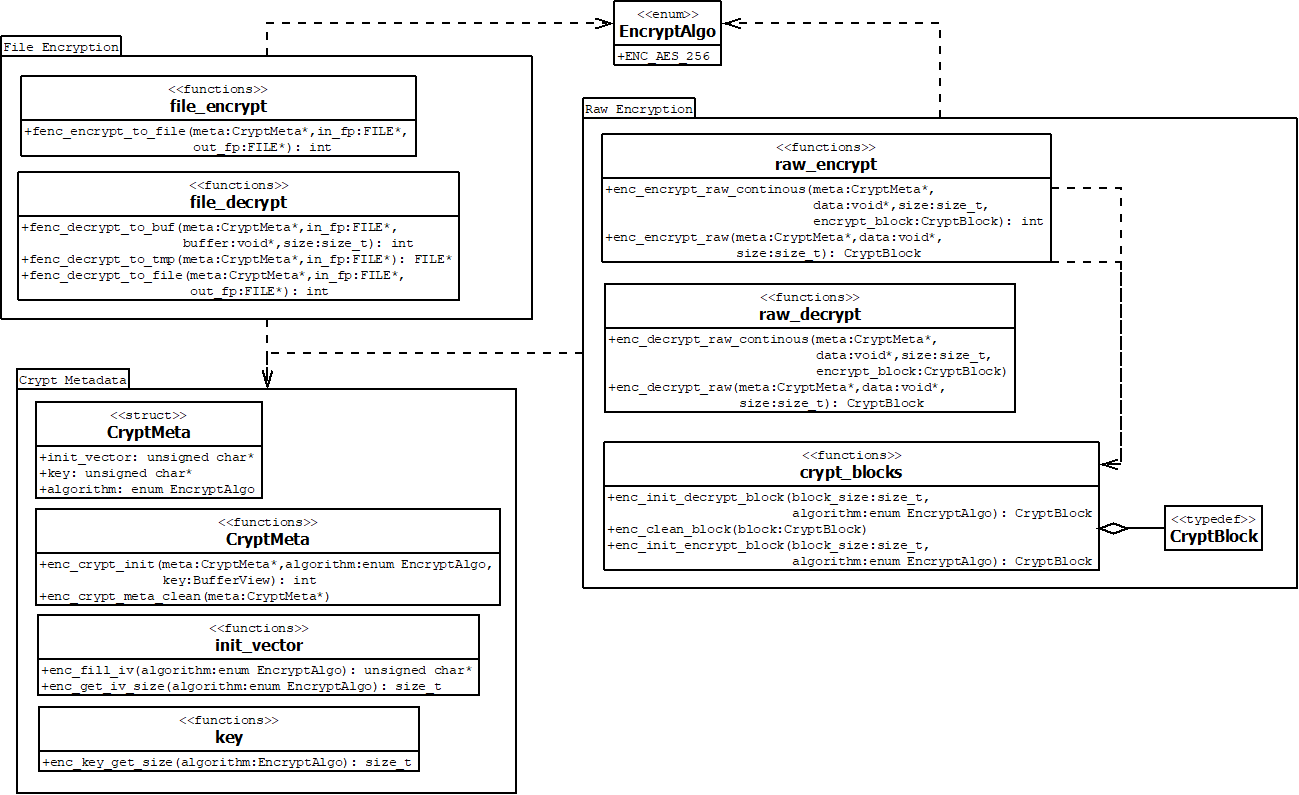
\includegraphics[scale=0.4]{\detaileduml/encrypt/encrypt}}
    \caption{Interfaces and design of the encryption components}
    \label{dia:encrypt_design}
\end{figure}

The class diagrams of figure \ref{dia:encrypt_design} show that the file
encryption side offers quite a minimal interface compared to the raw encryption
side. This is because data encryption itself holds a lot of implementation
details (initialization vectors, different block sizes etc.) that need not to
be revealed when all the user wants to do is encrypt or decrypt a file.

The basic idea of the design is that the user provides the password database
(file) that he wants to encrypt, algorithm and the key that will be used. From
here the implementation will construct the \texttt{CryptMeta} object that is
used with the raw encryption functions, which will contain the key, the
initialization vector, and the requested algorithm.

Then, depending on the size of the requested file encryption/decryption
the functions will either construct a reusable \texttt{CryptBlock} with an
optimal size, or use the one-time encrypt/decrypt functions provided by the
interface (continous and non-continous). The continous ones were designed
to accomodate extremely large databases, where constantly allocating and
deallocating new blocks would not be feasible.

\subsection{Database handling}
\subsection{Hashing}

Hashing inherits many of the same design aspects from encryption, as the
operations are quite similar with, of course, hashing being quite simpler.
The design of the hashing component can be seen in \ref{dia:hash_design}.

\begin{figure}[H]
    \centering
    \centerline{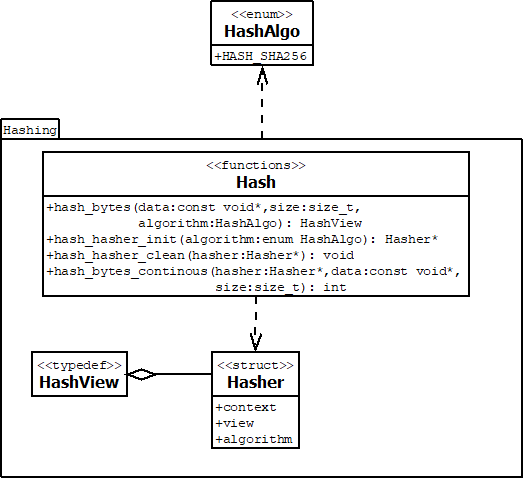
\includegraphics[scale=0.55]{\detaileduml/hash/hash}}
    \caption{Interfaces and design of the hashing component}
    \label{dia:hash_design}
\end{figure}

Both one-time and continous hashing are supported as with encryption. The user
will either construct a \texttt{Hasher} object to support continous hashing, or
use the one-time hashing provided with function \texttt{hash\_bytes}.

\subsection{Authentication}
\subsection{Persistence}
\subsection{Options}
\subsection{User input}
\subsection{Logging}
